% XCircuit output "E:/6. SPRING 2022/EE236/GitHub/EE236-Lab/Labs/Lab 6/b.eps.tex" for LaTeX input from E:/6. SPRING 2022/EE236/GitHub/EE236-Lab/Labs/Lab 6/b.eps.ps
\def\putbox#1#2#3{\makebox[0in][l]{\makebox[#1][l]{}\raisebox{\baselineskip}[0in][0in]{\raisebox{#2}[0in][0in]{#3}}}}
\def\rightbox#1{\makebox[0in][r]{#1}}
\def\centbox#1{\makebox[0in]{#1}}
\def\topbox#1{\raisebox{-\baselineskip}[0in][0in]{#1}}
\def\midbox#1{\raisebox{-0.5\baselineskip}[0in][0in]{#1}}
\begin{flushleft}
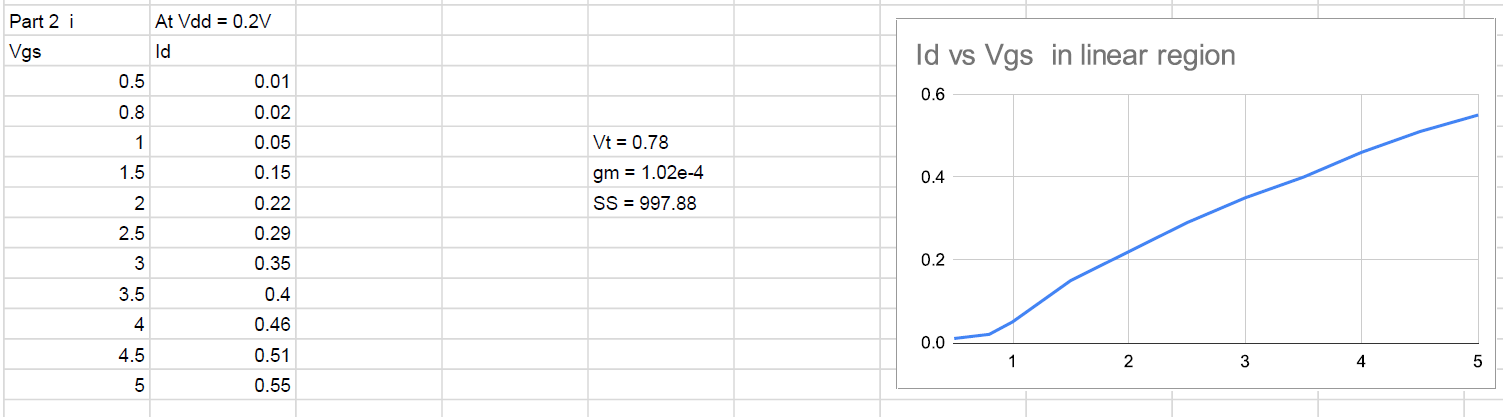
\epsfig{file=E:/6. SPRING 2022/EE236/GitHub/EE236-Lab/Labs/Lab 6/b.eps.ps}\\
% translate x=599 y=448 scale 0.38
\putbox{0.43in}{1.06in}{\centbox{\midbox{125MHz}}}%
\putbox{0.93in}{0.06in}{CMOS Inverter}%
\end{flushleft}
